Recently, I've been getting into graph theory with my interest in competitive
programming and other math problems \MarginComment{Hopefully you'll see more of
this quite soon ;)}, and one day I had the idea of creating an animation of
what \textit{all} the (undirected, without loops) graphs look like for some \(
n \) vertices, and creating some aesthetically pleasing looking visualization
that moves between all of them. This journal entry was really inspired by the
math that goes behind it and how one actually goes about (somewhat) efficiently
generating these graphs.

The end result ended up turning out to be quite nice (at least in my opinion)
even if it was quite a simple visualization in idea. You can check it out here:
\url{https://chirprush.github.io/animations/animations/graph-iterations/index.html}.

\subsection{Encoding Graphs}

The idea that was sort of swimming around in my head was how one would encode a
graph as something that could be easily manipulated and played around with. One
could take the simple route, storing a bunch of vertices and then collecting
all the edges as tuples holding the vertex information, but this is quite bulky
and certainly no fun, right? Surely we can compress a graph into something
smaller than that; We just first need to revisit what exactly makes a graph a
graph.

A graph is formally defined in terms of both its vertices and its edges, which
are connections between these vertices. For our purposes of seeing "all" graphs
though, we aren't really that concerned with the infinitely many positions of
these vertices, so we can just place them evenly spaced on a circle for
convenience and the visual appeal of \( n \)-gons. With vertices out of the
way, all that really determines our different graphs is the edges that connect
our \( n \) vertices. Since we're looking for a \textit{bijection} from some
space (which we'll call \( S \)) to this space of graphs, a good motivating
question is: for \( n \) vertices, how many graphs do we exactly have?

A simple combinatorial argument helps us out here. For each pair of vertices,
you can make the binary choice to either add an edge or leave it empty. Counting the number of possible pairs gives us
\begin{align*}
    \binom{n}{2} = \frac{n \left( n - 1 \right)}{2} \> \text{ possible pairs,} && \text{giving} && 2^{n \left( n - 1 \right) / 2} \> \text{ possible graphs}
.\end{align*}
This means that, for example, there are \( 2^3 = 8 \) total possible ways to
pick the edges on a graph with \( 3 \) vertices. Note that while this does
count graphs that are isomorphic to each other, including obvious "rotations," we're fine with this. After all, our goal is to show \textit{all} graphs.

\MarginComment{
    \begin{center}
        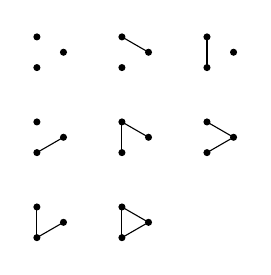
\begin{tikzpicture}[scale=0.9]
            \foreach \g in {0,...,7} {
                \foreach \i in {0,...,2} {
                    \node (\g\i) at ({1.2 * Mod(\g, 3) + 0.25 * cos(deg(\i * 2 * pi / 3))}, {-1.2 * floor(\g / 3) + 0.25 * sin(deg(\i * 2 * pi / 3))}) {};
                    \fill (\g\i) circle (0.05);
                }
            }

            \draw (10.center) -- (11.center);

            \draw (21.center) -- (22.center);

            \draw (30.center) -- (32.center);

            \draw (40.center) -- (41.center);
            \draw (41.center) -- (42.center);

            \draw (50.center) -- (51.center);
            \draw (52.center) -- (50.center);

            \draw (61.center) -- (62.center);
            \draw (62.center) -- (60.center);

            \draw (70.center) -- (71.center);
            \draw (70.center) -- (72.center);
            \draw (71.center) -- (72.center);
        \end{tikzpicture}
    \end{center}
    \captionof{figure}{All \( 8 \) possible graphs for \( 3 \) vertices.}
}

With this, we know our encoding must map from a set of \( 2^{n \left( n - 1
\right) / 2} \) elements to one unique graph, \textit{i.e.} \( \abs{S} = 2^{n
\left( n - 1 \right) / 2} \). We haven't really specified what the elements of
\( S \) should be, but one of the most useful and easy to work with choices is
simply the set of the integers \MarginComment{We will see later that this
choice to start counting from \( 0 \) is not merely because I'm a programmer.}
\[
    S = \{0, 1, \ldots, 2^{n \left( n - 1 \right) / 2} - 1 \}
.\]
This allows us to easily count up to some natural numbers and generate our
encoded graphs quite easily, which can then be decoded.

What we haven't yet chosen now is \textit{how} each number corresponds to a
graph and \textit{why}. There are quite a few ways of doing this (\( \abs{S}!
\), in fact), but we would like to choose one that makes both intuitive and
algorithmic sense. For this, we'll take a look a few steps back in our
approach, specifically to where we counted the number of graphs.

One structure associated with graphs that further illustrates the
\textit{binary} action of choosing whether or not to add an edge between two
vertices is an \textbf{adjacency matrix}. Recall that in graph theory, we
define the adjacency matrix of a simple graph to be an \( n \times n \) matrix
where each entry \( A_{ij} \) is either \( 1 \) if there exists an edge between
the \( i \)th and \( j \)th vertices and \( 0 \) if there does not. For example, for the graph \( C_4 \) (the cyclic graph with \( 4 \) vertices), the adjacency matrix is
\[
    A = \begin{bmatrix}
        0 & \tikzmark{tritop} 1 & 0 & \tikzmark{tricorn} 1 \\
        1 & 0 & 1 & 0 \\
        0 & 1 & 0 & \tikzmark{tribot} 1 \\
        1 & 0 & 1 & 0 \\
    \end{bmatrix}
.\]
\begin{tikzpicture}[remember picture, overlay]
    \fill[opacity=0.2, fadegray, rounded corners] ([xshift=-0.25cm, yshift=0.25cm]pic cs:tritop) -- ([xshift=0.2cm, yshift=0.25cm]pic cs:tricorn) -- ([xshift=0.2cm, yshift=-0.25cm]pic cs:tribot) -- cycle;
\end{tikzpicture}
Because this is a undirected graph, the matrix is symmetric about the diagonal,
and all we need to consider is one of the triangles (the one above or below the
diagonal). One can verify that this triangle has exactly the \( n \left( n - 1
\right) / 2 \) \MarginComment{A quick way to show this is that the diagonal
takes up \( n \) elements, so if we let \( T \) be the number of elements in
each triangle, we have \( 2T + n = n \times n \).} bits representing our edges.
Thus, we see something interesting here. If we \textit{flatten} the adjacency
matrix triangle, we can represent our graph as a number in binary form. This
also perfectly fits all our numbers into the domain set \( S \).

For example, in the case of the \( C_4 \) graph, we would encode it as \( G =
101101_2 = 45 \). Although in this case the number is a palindrome in base \( 2
\), we would place the bits according to the order they appear in the triangle.
The first bit (from the right) would correspond to the edge \( \set{1, 2} \),
the second corresponding to \( \set{1, 3} \), and so on.

With this, the animation also has the cool effect of sort of counting up in
binary with the edges. This also gives a somewhat natural progression from the empty graph to the complete graph for \( n \) vertices.

\MarginComment{
    \begin{center}
    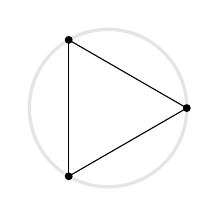
\begin{tikzpicture}
        \draw[opacity=0.1, very thick] (0, 0) circle (1);

        \node (v0) at ({1 * cos(0)}, {1 * sin(0)}) {};
        \node (v1) at ({1 * cos(deg(2 * pi / 3))}, {1 * sin(deg(2 * pi / 3))}) {};
        \node (v2) at ({1 * cos(deg(4 * pi / 3))}, {1 * sin(deg(4 * pi / 3))}) {};

        \fill (v0) circle (0.05);
        \fill (v1) circle (0.05);
        \fill (v2) circle (0.05);

        \draw (v0.center) -- (v1.center);
        \draw (v0.center) -- (v2.center);
        \draw (v1.center) -- (v2.center);
    \end{tikzpicture}
    \end{center}
    \captionof{figure}{The animation displaying the complete graph \( K_3 \), encoded as \( 111_2 = 7 \).}
}


Thus, we've found a suitable encoding for our graphs into numbers. In our
actual program, we're iterating over numbers and converting them to graphs
instead, so we'll also have to find some way of going the other way around.
Luckily, we've already built the foundation and intuition for how this will
work.

\subsection{Decoding Graph Numbers}

If the encoding stage involves taking a graph and turning it into a number
based on its adjacency matrix and edges, the decoding stage is precisely the
opposite of this: we take a number, decompose it into it's binary
representation, and turn it into an adjacency matrix, which defines the edges
and the complete representation of our graph.

There are quite a few ways do this, but in order to choose a sensible one,
we'll look at the edges of the graphs, specifically the vertices that they
connect. If we number (quite arbitrarily) the vertices of a graph \(
1,2,\ldots,n \), we have the following unique (undirected) edges:
\[
\begin{array}{cccc}
    \set{1, 2}, & \set{1, 3}, & \cdots, & \set{1, n} \\
    \set{2, 3}, & \cdots, & \set{2, n} & \\
    \vdots & \udots & \\
    \set{n - 1, n} & & &
\end{array}
\]
We want each bit of our "number to be decoded" to correlate to an edge in this
triangle, and to do so, we work from right to left in the binary representation
of the number. If the \( b \)th bit from the right is \( 1 \), we draw in the
\( b \)th edge identified in this triangle. Mathematically, we can express this as a fairly straightforward-to-follow algorithm,
\begin{blackbox}
    \begin{algorithmic}
        \State \texttt{/*}
        \State \texttt{\ \ \ We let n denote the number of vertices and b be a value from}
        \State \texttt{\ \ \ 1 to n(n - 1)/2 representing an edge and a bit in graph number. */}
        \Function{GetEdge}{$n, b$} % Bruhhhhhh I seriously have to do this
            \For{\( i \) in \( 1,\ldots,n - 1 \)}
                \If{\( b \le n - i \)}
                    \State \Return \( \set{i, b + i} \)
                \Else
                    \State \( b \gets b - \left( n - i \right) \)
                \EndIf
            \EndFor
        \EndFunction
    \end{algorithmic}
\end{blackbox}
or a closed form expression of which I shall omit the derivation
\MarginComment{I mostly derived the closed form because I thought it would be
just a bit fun. For anyone curious on how I arrived at it, one can recall
the formula for the sum of the first \( n \) natural numbers. If we set
this equal to a number, floor the result, we obtain the formula with a bit
of work.} because it's a bit cumbersome and rather uninteresting. Let \( k = n \left( n - 1 \right) / 2 - b \). Then we have edge \( \set{i, j} \) where
\begin{align*}
    i &= 1 + \floor{\left( n - 1 \right) - \left( \sqrt{1 + 8k} - 1 \right) / 2}, \\
    j &= 1 + i + b - \left( i - 1 \right) \left( 2n - i \right) / 2
.\end{align*}
And with this, we have pretty much most of the logic behind the graph iteration
animation (well, besides the drawing logic, which is cool although not the most
mathy). Be sure to check it out! I think it came out quite well.
